\chapter{Rendering and Color Science}
\label{chap:render}

This chapter serves as an introduction to computer graphics and color science. We briefly overview basic aspects of these fields, mainly to familiarize the reader with some of the fundamental processes, their backgrounds, and usages. We also establish the terminology, such as \emph{rendering} or \emph{RGB color space}, that will be used throughout the thesis frequently. A significant part of the following sections is based on the publications by~\citet{wyszecki1982color},~\citet{colorScienceSlides},~\citet{nimier2019mitsuba} and~\citet{pharr2016physically}.

First, we discuss the mechanisms behind the light and colors and then we look into the process of the physically-based image synthesis.

\section{Light}

According to the definition by \citet{barbrow1964international}, the light is "any radiation capable of causing a visual sensation directly". In other words, a visible light is electromagnetic radiation that is perceivable by human eye. 

As all electromagnetic radiations, the light also propagates in form of waves. The oscillation direction of these waves does not change the color of the light. However, it may interact differently with reflective/refractive objects as it passes through them. A representation of such wave propagation is displayed in \autoref{fig:wave}.

\begin{figure}[h]
	\centering
	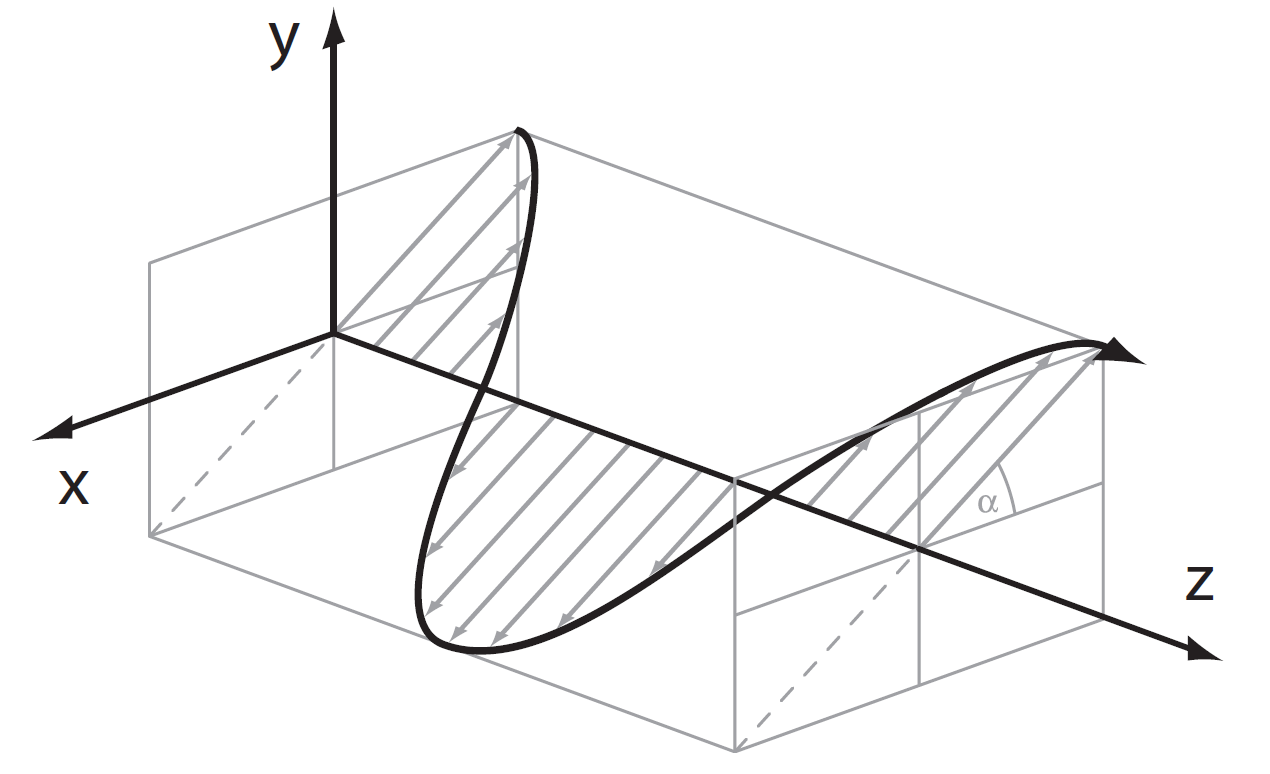
\includegraphics[width=0.7\linewidth]{img/wave.png}
	\caption{A propagation of wave~\cite{colorScienceSlides}}
	\label{fig:wave}
\end{figure}


Usually, by the term light, we mean the visible light which consists of multiple waves of unique frequencies (wavelengths). There are no exact boundaries to the visible spectrum as distinct human eyes might perceive light slightly differently. The lower boundary is estimated between 360 and 400nm and the upper boundary from 760 to 830nm~\cite{sliney2016light}. The light above this range is called infrared light and below ultraviolet. An explanatory image of the known electromagnetic wavelengths can be found in \autoref{fig:wavelengths}.

\begin{figure}[h]
	\centering
	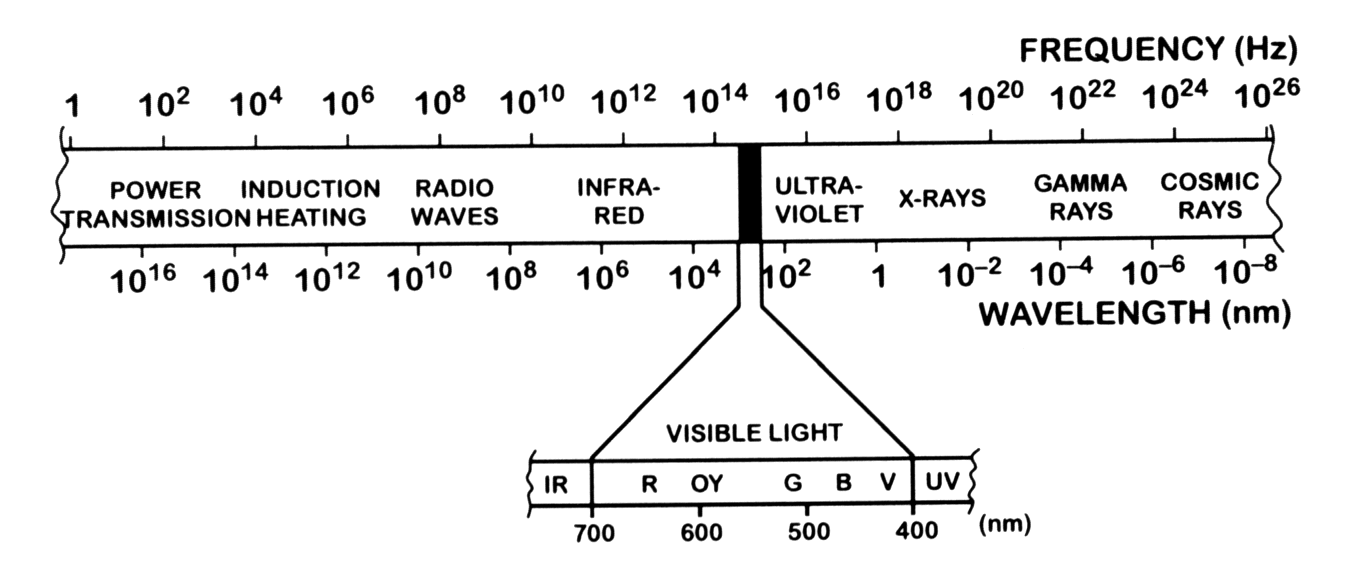
\includegraphics[width=0.8\linewidth]{img/wavelengths.png}
	\caption{An image displaying various wavelengths~\cite{colorScienceSlides}}
	\label{fig:wavelengths}
\end{figure}

\subsection{Color}

While observing an illuminated object, three different signals are sent from the eye sensors (rods and cones) to the brain, each representing either a red, a green, or a blue channel. When put together inside the brain, they form a sensation of the color. 

To categorize the colors, several reproducible representations were formed, called the \emph{color spaces}. A natural decision was to create an \emph{RGB color space} as it directly correlates with the signals sent from the human eyes' rods and cones. Note that multiple variations of the RGB color space exist, such as \emph{sRGB} or \emph{Adobe RGB}. An illustrative comparison between several color gamuts is shown in \autoref{fig:gamut}.

\begin{figure}[h]
	\centering
	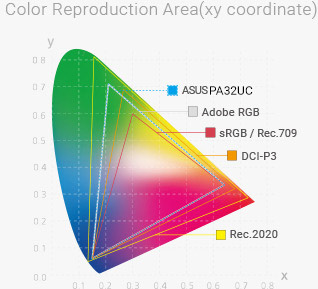
\includegraphics[width=0.6\linewidth]{img/gamut.jpg}
	\caption[ASUS RGB]{An illustrative comparison between five RGB gamuts by Asus \footnotemark}
	\label{fig:gamut}
\end{figure}
\footnotetext{\url{https://www.asus.com/Microsite/ProArtMonitor/experience-truecolor.html}}

In 1913, the Commission internationale de l'éclairage (International Commission on Illumination), shortly CIE, was formed as an authority that defines almost everything that concerns colors and their perception. In 1931, they conducted color matching experiments to obtain three color matching functions that would convert the color stimuli perceived in our eyes to the \emph{CIE RGB} color space. As these functions had a negative component, a new imaginary color space was created, called \emph{CIE XYZ}. These conversions are further described in \autoref{conversion}.

CIE also defined \emph{CIE L*a*b*} color space, standard illuminants D65 and D50 and many others.

\subsection{Conversions to tristimulus color spaces}
\label{conversion}

The conversion from a spectrum to an RGB color space looks as follows:

\begin{enumerate}
	\item Compute the tristimulus value XYZ using the CIE color matching functions (shown in \autoref{fig:cmf})
	\begin{align*} 
	X=\int P(\lambda)\overline{x}(\lambda)d\lambda\\
	Y=\int P(\lambda)\overline{y}(\lambda)d\lambda\\
	Z=\int P(\lambda)\overline{z}(\lambda)d\lambda
	\end{align*} 
	, where $P(\lambda)$ is the spectral power distribution and $\overline{x}(\lambda)$, $\overline{y}(\lambda)$ and $\overline{z}(\lambda)$ are the color matching functions.
	\item Convert the XYZ to the desired RGB color space using a transformation matrix. The matrix differs depending on the specific RGB color space --- an example of CIE XYZ to sRGB conversion:
	\begin{align*}
	r=3.240X-0.969Y+0.55Z\\
	g=-1.537X+1.875Y-0.204Z\\
	b=-0.498+0.041Y+1.057Z
	\end{align*}
	\item (Optional) As the resulting r,g,b values may be negative, a gamut mapping might be necessary.
\end{enumerate}

\begin{figure}[httpb]
	\centering
	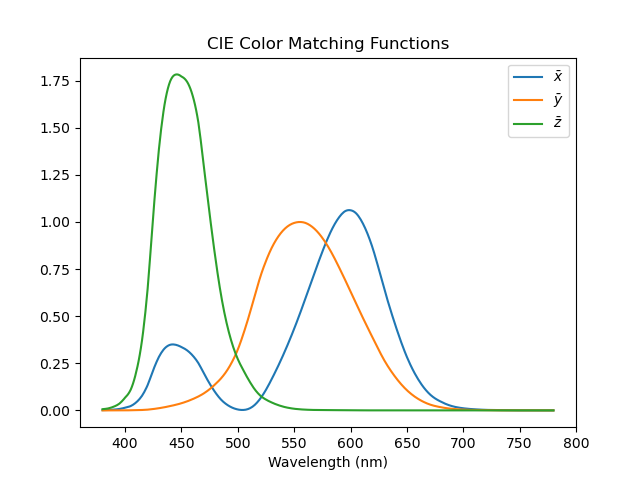
\includegraphics[width=.8\linewidth]{img/cmf.png}
	\caption[CMF]{Color matching functions plotted in Python\footnotemark}
	\label{fig:cmf}
\end{figure}
\footnotetext{The (X,Y,Z) data are taken from \url{https://www.waveformlighting.com/tech/color-matching-function-x-y-z-values-by-wavelength-csv-excel-format}}

\subsection{Photometry and Radiometry}

Two different sets of measurement units were developed to quantify the light --- \emph{photometry} and \emph{radiometry}. Radiometry recognizes the light as an electromagnetic radiation while photometry focuses on the human perception of the light. Despite the distinct purposes, their quantities are often easily convertible. The following table shows some of their basic quantities:

\begin{tabular}{ll}
	\hline
	\textbf{Radiometric Quantity} & \textbf{Photometric Equivalent} \\
	\hline \hline
	Spectral radiant energy [$J$] & Luminous energy [$Lumen-second$] \\
	\hline
	Radiant flux [$W$] & Luminous flux [$Lumen$] \\
	\hline
	Irradiance [$W.m^{-2}$] & Illuminance [$Lumen.m^{-2}$]  \\
	\hline
	Radiant intensity [$W.sr^{-1}$] & Luminous intensity [$candela=Lumen.sr^{-1}$] \\
	\hline
	Radiance [$W.sr^{-1}.m^{-2}$] & Luminance [$candela.m^{-2}$]
\end{tabular}

Each of these quantities is briefly mentioned in the following description:
\begin{description}
	\item[Spectral radiant energy] Amount of light energy at a specific wavelength
	\item[Radiant flux] Amount of light energy with respect to time
	\item[Irradiance] Flux at a specific point (space)
	\item[Radiant intensity] Flux in a direction (steradian, shortly $sr$, is a unit of the solid angle --- a surface on a unit sphere, the whole sphere has $4\pi$ steradians)
	\item[Radiance] Spatial and directional flux
\end{description}

The relationship between these quantities is described by the \emph{spectral efficiency function}. It states how efficiently a human eye reacts to different wavelengths, implying that some wavelengths are detected more easily. As we can see in \autoref{fig:lum}, the scotopic (night) perception peaks at around 507nm and the photopic (day) perception at 555nm.

\begin{figure}[h]
	\centering
	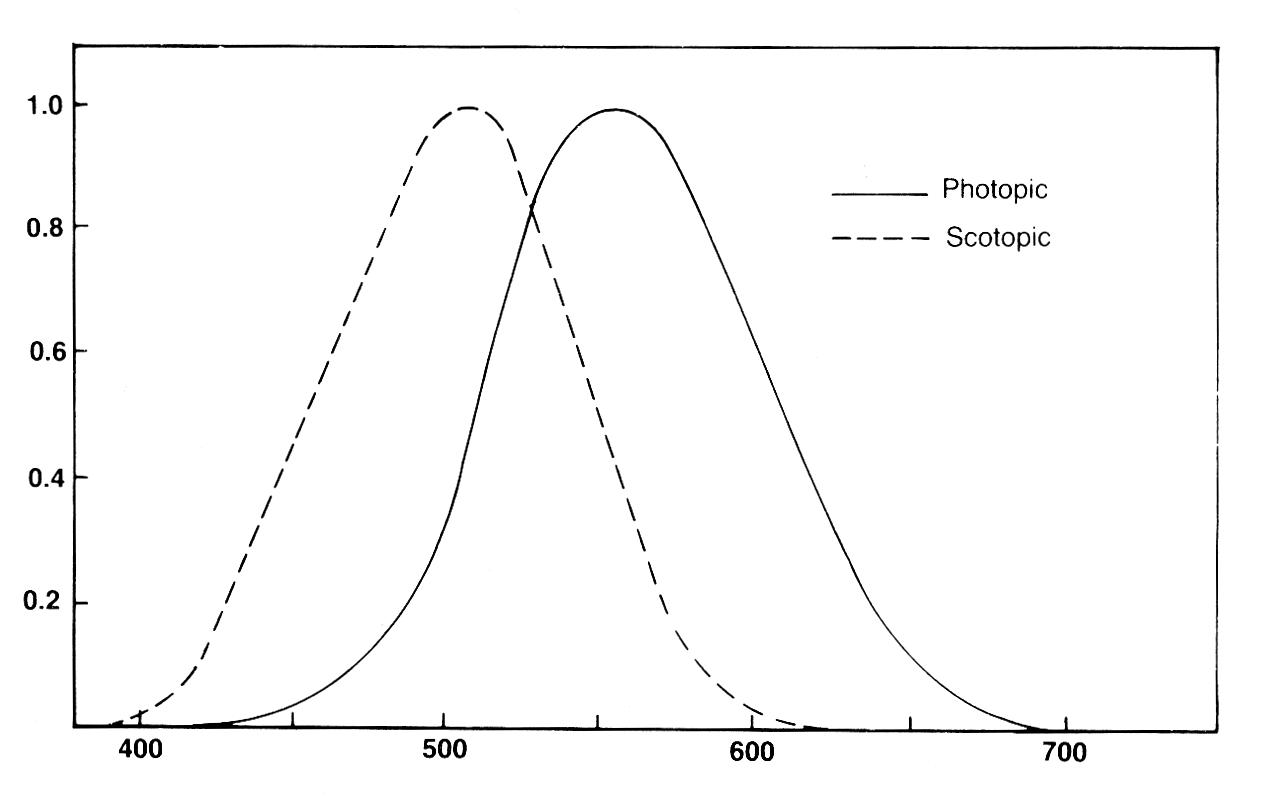
\includegraphics[width=0.8\linewidth]{img/luminous_efficiency.png}
	\caption{Relative luminous efficiency function~\cite{colorScienceSlides}}
	\label{fig:lum}
\end{figure}

\section{Physically based rendering}

One of the ultimate goals of computer graphics is the ability to reproduce visually plausible and physically coherent images that should be indistinguishable from a photograph. Such a process is called \emph{photorealistic rendering}. In this thesis, we abbreviate the term and call it simply \emph{rendering} as the non-photorealistic one does not concern us.

The main job of a rendering system (\emph{renderer}) is to simulate various phenomena commonly seen in nature, such as light reflections, refractions, shadows, etc, accurately to their physical models. Nowadays, modern renderers are capable of recreating the scenes so authentically that the rendered images are almost identical to real-life photos. An example can be seen in \autoref{fig:corona_render}.

\begin{figure}[h]
	\centering
	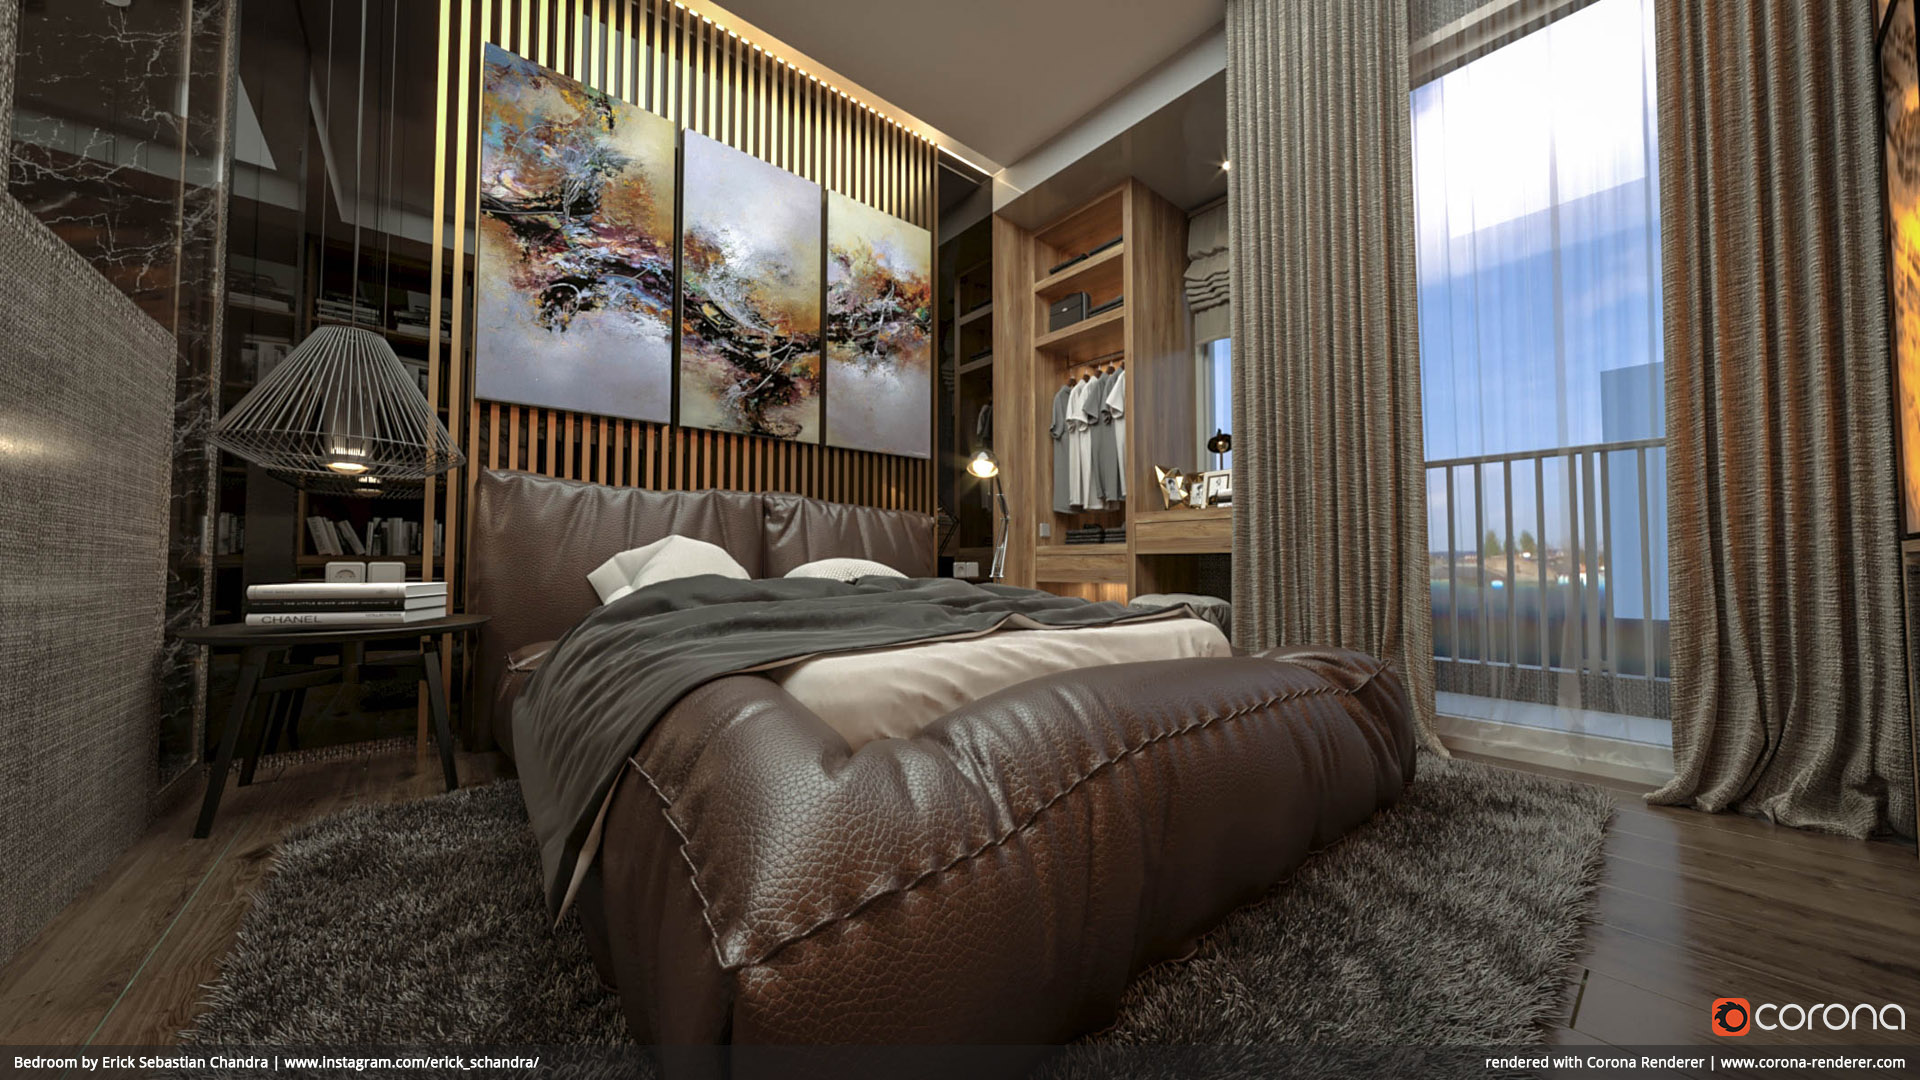
\includegraphics[width=\linewidth]{img/corona_render.jpg}
	\caption[Corona image]{An image generated with the Corona Renderer\footnotemark}
	\label{fig:corona_render}
\end{figure}
\footnotetext{\url{https://corona-renderer.com/gallery}}

The rendering workflow is similar for every renderer:
\begin{enumerate}
	\item A 3D digital scene is described by the objects it contains
	\item A light simulation algorithm runs for every visible pixel from the viewer
	\item Upon object interaction, the shading of the intersected point is computed
	\item As the algorithm terminates, an image ("photograph") of the scene called the \emph{render} is created
\end{enumerate}

This process is further explained in \autoref{sec:light_transport}.

\subsection{Digital scene}

Basic elements of a digital scene are roughly the same for each renderer:

\begin{description}
	\item[Camera] A camera (or a sensor) in a digital scene works in the same manner as in real life --- it records a picture. Generally, it is possible to define the coordinate position and the viewing vectors but also the properties such as focal distance or the type of the film.
	\item[Light source] The scene needs to be illuminated by at least on light source to be visible. The common types of lights are point light, area light, spotlight, and environment (constant) light. 
	\item[Objects] The visible contents of the scene are objects. Almost all rendering systems offer a choice to either use their prepared basic geometry, such as spheres and triangles or to include a mesh geometry from an external file (usually created by a modeling software). These objects must state their material properties so that the algorithm may correctly interact with them, e.g. diffuse vs. reflective material.
\end{description}

Unfortunately, as each renderer may have unique implementation details, the formats of the scenes are vastly different. For example, mitsuba uses XML, but PBRT has its specific format. An example of a simple scene for Mitsuba2 can be found in \autoref{fig:example_scene}.

\definecolor{maroon}{rgb}{0.5,0,0}
\definecolor{darkgreen}{rgb}{0,0.5,0}
\lstdefinelanguage{XML}
{
	basicstyle=\ttfamily,
	morestring=[s]{"}{"},
	morecomment=[s]{?}{?},
	morecomment=[s]{!--}{--},
	commentstyle=\color{darkgreen},
	moredelim=[s][\color{black}]{>}{<},
	moredelim=[s][\color{red}]{\ }{=},
	stringstyle=\color{blue},
	identifierstyle=\color{maroon}
}

\begin{figure}[httpb]
\begin{tabular}{p{0.3\textwidth}p{0.6\textwidth}}
\begin{minipage}{0.3\textwidth}
	
\includegraphics[width=\linewidth]{img/example_scene.png}
\end{minipage}
	&
\begin{minipage}{0.6\textwidth}
	\lstset{language=XML}
	\begin{lstlisting}[basicstyle=\tiny]
<scene version="2.0.0">
 <!-- Light transport algorithm -->
 <integrator type="path"/>
	
 <!-- Camera looking at the sphere -->
 <sensor type="perspective">
  <transform name="to_world">
   <lookat origin="0,-6,0" target="0,0,0" up="0,0,1"/>
  </transform>
 </sensor>
	
 <!-- Red sphere in the middle -->
 <shape type="sphere">
  <bsdf type="diffuse">
   <rgb name="reflectance" value="1.0,0.0,0.0"/>
  </bsdf>
 </shape>
	
 <!-- Light blue light all around the scene-->
 <emitter type="constant">
  <rgb name="radiance" value="0.6,0.8,0.9"/>
 </emitter>
</scene>
	\end{lstlisting}
\end{minipage}
\end{tabular}
\caption{A simple scene rendered with Mitsuba2 (left) along with its scene description (right)}
\label{fig:example_scene}
\end{figure}

Once the scene is described, the renderer runs a light transport simulation inside it to determine the colors of the final image. As this is a fundamental part of the rendering process, the following sections describe the physics theory and the models behind the light transport and the materials.

\subsection{BRDF}
\label{sec:BRDF}

The reflective properties of a material are described by \emph{Bidirectional Distribution Reflectance Function}, shortly \emph{BRDF}~\cite{nicodemus1965directional}. Its equation looks as follows:

\begin{equation} \label{eq:brdf}
f_r(\omega_i,\omega_o)=\frac{dL_o(\omega_o)}{L_i(\omega_i)cos\theta_i d\omega_i}
\end{equation}

Essentially, it states how much radiance is reflected from the incoming direction $\omega_i$ ($L_i(\omega_i)$) to the outgoing direction $\omega_o$ ($L_o(\omega_o)$) for a specific material.
An image interpretation of the function is in \autoref{fig:brdf}. As it is a distribution function, we can also reformulate its meaning as a probability density that a defined amount of light energy gets reflected from $\omega_i$ to $\omega_o$.

\begin{figure}[h]
	\centering
	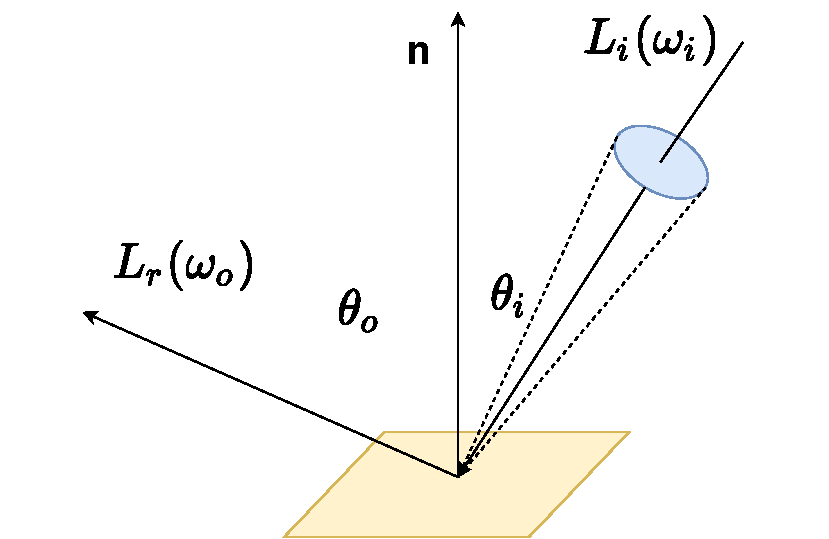
\includegraphics[width=85mm]{img/brdf.pdf}
	\caption{Bidirectional Distribution Reflectance Function}
	\label{fig:brdf}
\end{figure}

In the simplest cases, BRDF describes the reflectivity of a surface. Renders of a diffuse, a glossy, and a mirror material are compared in \autoref{fig:compare_brdf}.

\begin{figure}[httpb]
	\begin{tabular}{ccc}
		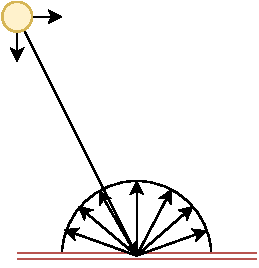
\includegraphics[width=.3\linewidth]{img/brdf_diffuse_diag.pdf}
		&
		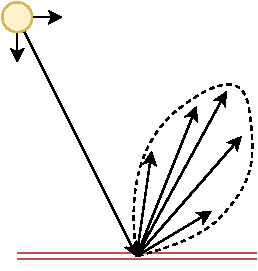
\includegraphics[width=.3\linewidth]{img/brdf_glossy_diag.pdf}
		&
		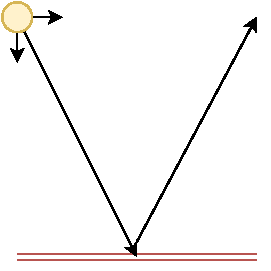
\includegraphics[width=.3\linewidth]{img/brdf_mirror_diag.pdf} \\
		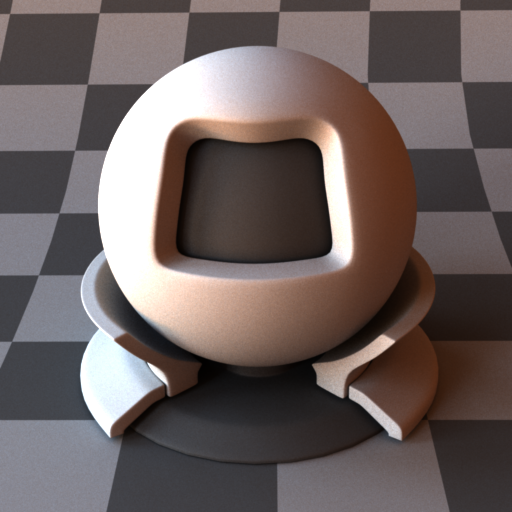
\includegraphics[width=.3\linewidth]{img/brdf_diffuse.png}
		&
		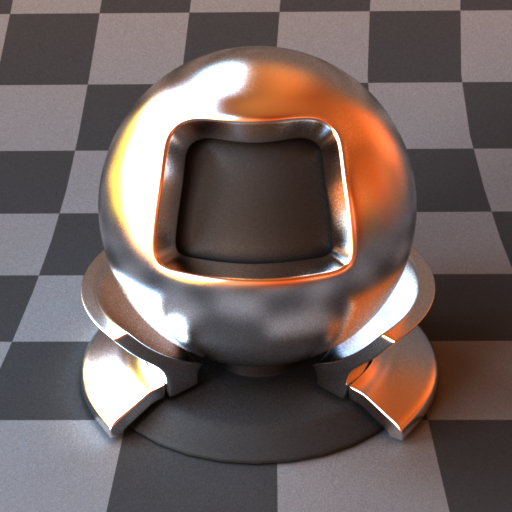
\includegraphics[width=.3\linewidth]{img/brdf_glossy.png}
		&
		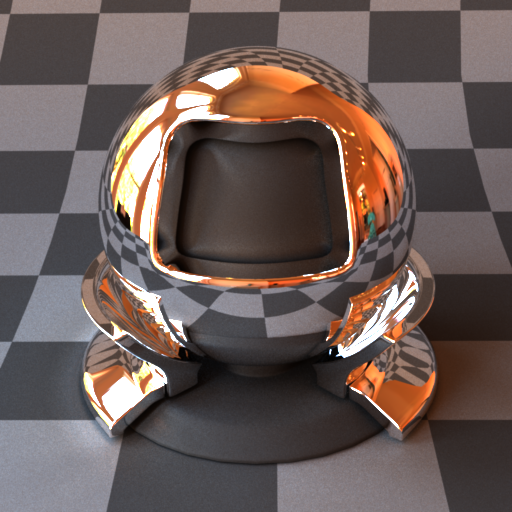
\includegraphics[width=.3\linewidth]{img/brdf_mirror.png}
	\end{tabular}
	\caption{A preview of a diffuse (left), a glossy (middle) and mirror (right) material rendered in Mitsuba2 along with their illustrative BRDF visualizations}
	\label{fig:compare_brdf}
\end{figure}


Physically-based BRDFs must fulfill the following properties~\citealp{duvenhage2013numerical}:
\begin{description}
	\item[Helmholtz reciprocity] The amount of reflected energy from the incoming direction to the outgoing direction is equal to the amount of energy in reversed directions ($f_r(\omega_i,\omega_o)=f_r(\omega_o,\omega_i)$).
	\item[Energy conservation] The amount of reflected energy cannot be greater than all received energy.
	\item[Positivity] BRDF is always positive ($f_r(\omega_i,\omega_o)\ge0$).
\end{description}

Note that BRDF concerns only opaque surfaces. There exist multiple distribution functions that describe the behavior of other materials, for example:
\begin{description}
	\item[BTDF] Describes light transmission
	\item[BSDF] Combination of BTDF and BRDF (e.g. glass, water)
	\item[BSSRDF] Considers scattering of the light under the surface (e.g. skin)
\end{description}

In this thesis, most of the materials that we talk about are described by BSDFs.

\subsection{Global Illumination}

With the BRDF defined, we can now formulate an equation that evaluates the global illumination of a scene, which is the illumination of each point from all light sources. It is generally called the \emph{rendering equation}~\cite{kajiya1986rendering} and it can be computed as follows:

\begin{equation}
L_o(x,\omega_o)=L_e(x,\omega_o)+L_r(x,\omega_o)
\end{equation}

, where:
\begin{description}
	\item[$x$] is the currently computed point in the scene.
	\item[$L_o$] is the outgoing radiance.
	\item[$L_e$] is the radiance emitted by $x$ as $x$ can be on a light source.
	\item[$L_r$] is also called the \emph{reflectance equation} and it states the total amount of the reflected radiance for all contributions of the incident radiance. Hence, it is an integral over the upper hemisphere over $x$ that is denoted as follows:
	\begin{equation}
	L_r(x,\omega_0)=\int_{\Omega}f_r(x,\omega_o,\omega_i) L_i(x,\omega_,i) cos\theta_i d\omega_i
	\end{equation}
	, where
	\begin{description}
		\item[$f_r(x,\omega_o,\omega_i)$] is the BRDF of $x$ as defined in \autoref{eq:brdf}.
		\item[$L_i(x,\omega_i)$] is the incoming radiance from a light source.
	\end{description}
\end{description}

An image interpretation of the reflectance equation can be seen in \autoref{fig:refl}.

\begin{figure}[h]
	\centering
	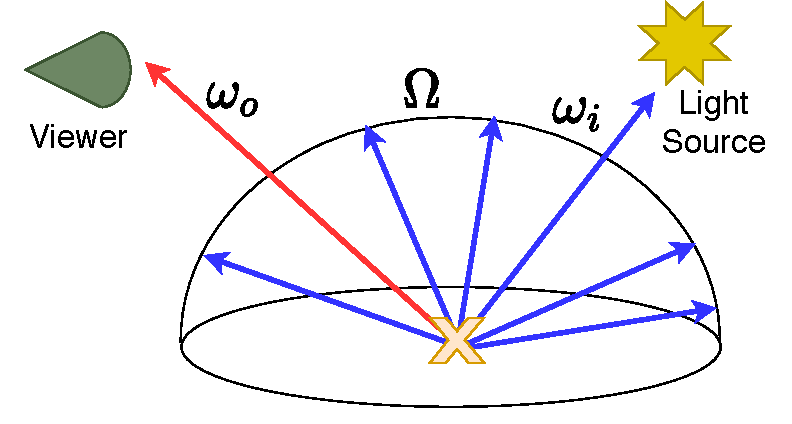
\includegraphics[width=85mm]{img/refl.pdf}
	\caption{Reflectance Equation}
	\label{fig:refl}
\end{figure}

Every light transport algorithm tries to solve some of the formulations of the rendering equation.

Interestingly, the light transport is recursive in nature. As we can see from the rendering equation, to compute the outgoing radiance at a certain point $x$, we need to know all the contributing incoming radiances. These do not necessarily have to originate at a light source --- the incoming radiance may come from another, non-emitting point $y$ in the scene as a result of the rendering equation computed at the point $y$.

\subsection{Monte Carlo integration}
Before we proceed to the actual algorithms that evaluate the rendering equation, we briefly introduce a method that is used to approximate the definite integral --- \emph{Monte Carlo integration}~\cite{caflisch1998monte}.

Formally, for a multidimensional definite integral
\begin{equation}
I=\int_{\Omega}g(x)dx
\end{equation}
 Monte Carlo (MC) estimates I as 
 \begin{equation}
 \langle I\rangle=\frac{1}{N}\sum_{k=1}^{N}\frac{g(\xi_k)}{p(\xi_k)}; \xi_k\propto p(x)
 \end{equation}

\begin{figure}[H]
	\centering
	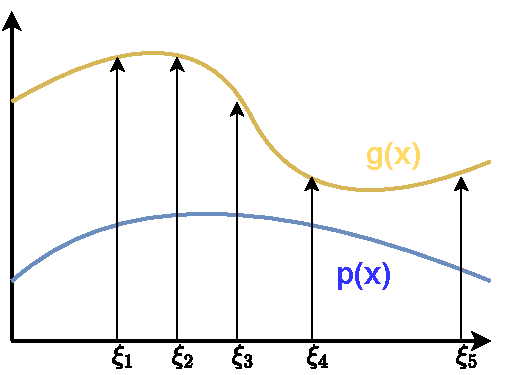
\includegraphics[width=0.5\linewidth]{img/monte_carlo.pdf}
	\caption{Monte Carlo method 2D visualization}
\end{figure}

In other words, Monte Carlo is a non-deterministic method that sums N randomly chosen samples $\xi_k$, computes their values $g(\xi_k)$, and averages them. To reduce variance, importance sampling is introduced by drawing samples from a distribution $p(x)$ that is chosen for each specific problem to approximate the former $g(x)$ function. In reality, importance sampling ensures that if some samples are generated twice as much, their weight is decreased by half.

There exist other methods that are used to approximate integrals, such as deterministic quadrature or Markov Chain Monte Carlo (MCMC).

\subsection{Light transport algorithms}
\label{sec:light_transport}

\subsubsection{Path tracing}
Over the years, a large number of various light transport algorithms and their variations have been developed, where each has its own benefits. The one that we mention the most in this thesis is called the \emph{path tracing}. Its core idea is simple:

\renewcommand{\labelenumii}{\theenumii}
\renewcommand{\theenumii}{\theenumi.\arabic{enumii}.}
\begin{enumerate}
	\item For each pixel in the image plane, shoot a primary ray $r$ from the camera into the scene.
	\item If $r$ hits a non-emitting object at point $x$:
	\begin{enumerate}
		\item Compute BRDF at $x$.
		\item Generate a new random direction $\omega$. Ideally, the distribution of the generated direction should be proportional to the BRDF --- e.g. diffuse BRDF generates a direction uniformly over a hemisphere while glossy BRDF prioritizes samples from the reflectance lobe (shown in \autoref{fig:compare_brdf}).
		\item Add the BRDF value to the final color of the pixel.
		\item Check for a terminating condition. There exist several options, usually, a combination of them is applied:
			\begin{description}
				\item [Maximum depth] A user specified maximum number of recursions.
				\item [Russian Roulette] Randomly choose if the ray survives, lowering the chance with each consecutive bounce.
				\item [BRDF-proportional] Depending on the surface material, decide \\ whether the ray survives or not. For example, reflective or refractive surfaces need a lot more recursions as they propagate the light further into the scene than diffuse surfaces.
			\end{description}
		\item In case the termination was not successful, bounce -- shoot a secondary ray $r$ from the point $x$ in the direction $\omega$ and go to step 2.
	\end{enumerate}
	\item If $r$ hits an emitting object (light source), add its emission $L_e$ to the final color of the pixel
	\item If no scene geometry is hit, terminate the algorithm and add the color of the surrounding light (if there is any).
\end{enumerate}

The bouncing of the light in the scene correlates with the recursive nature of the rendering equation. Even though the path tracing is a slow algorithm (i.e. not suitable for real-time rendering in games), its variations can be extremely accurate. Providing equally accurate surface models used in the scene, the resulting images might even be indistinguishable from real photographs. 


\paragraph{MIS}

In the algorithm described above, the direct illumination computation of each scene intersection is dependent only on the BRDF of the intersected surface and the consequent walk to the light source. Ideally, each walk should end by hitting a light source, which depends on the number of samples and the maximum allowed depth of the recursion. Consequently, this creates variance which can be easily improved by the integration of the \emph{multiple importance sampling} (MIS). Generally, it involves a weighted combination of multiple sampling techniques. Typically, it combines the BRDF proportional sampling and the light source sampling --- in each step of the path tracing, every light source that is visible from the intersected point contributes to point's value. Both sampling methods are obviously, weighted to avoid over-illumination. 

\paragraph{Volumes}

Another aspect that needs to be accounted for in the rendering process are volumetric objects, such as fogs or smokes. Typically, there are two ways that a volumetric object may affect the light passing through it. The volume can attenuate the light by absorbing it or scattering it to different directions. But, the volume can also strengthen the light by emitting light (e.g. flame) or scattering light from different directions to the sampled one.

A single walk of a path tracer capable of volume tracing and MIS sampling is visualized in \autoref{fig:path_tracer_vis}.

\renewcommand\thesubfigure{\arabic{subfigure}}
\begin{figure}
	\begin{tabular}{cc}
		\begin{subfigure}
			{0.45\textwidth}\centering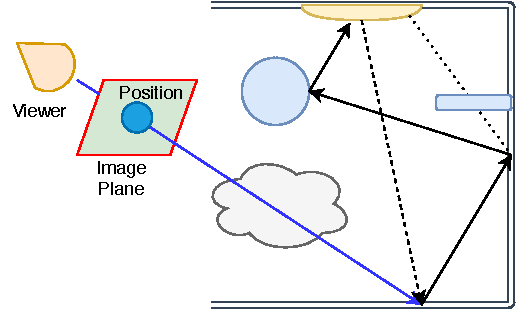
\includegraphics[width=\linewidth]{img/path_tracer_step1.pdf}
			\caption{Primary ray created}
		\end{subfigure}
		&
		\begin{subfigure}
			{0.45\textwidth}\centering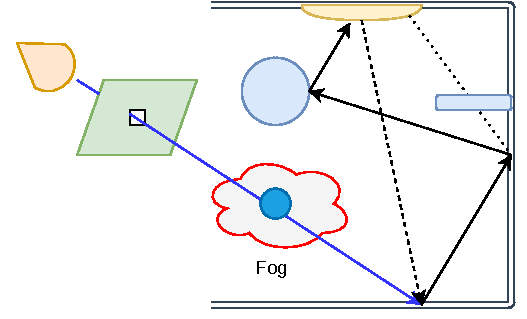
\includegraphics[width=\linewidth]{img/path_tracer_step2.pdf}
			\caption{Passing volume, attenuation}
		\end{subfigure} \\
		\begin{subfigure}
			{0.45\textwidth}\centering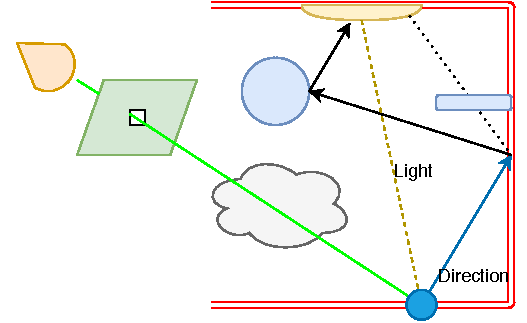
\includegraphics[width=\linewidth]{img/path_tracer_step3.pdf}
			\caption{ Geometry hit, new direction, BRDF + light added}
		\end{subfigure} 
		&
		\begin{subfigure}
			{0.45\textwidth}\centering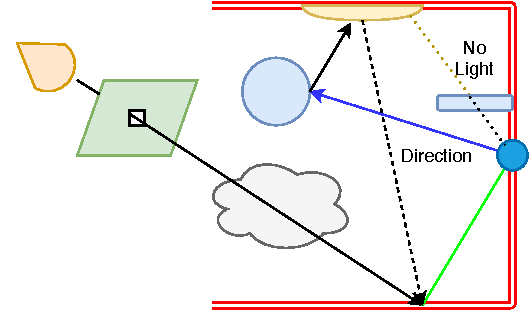
\includegraphics[width=\linewidth]{img/path_tracer_step4.pdf}
			\caption{Geometry hit, new direction, BRDF added (light obscured)}
		\end{subfigure} \\
		\multicolumn{2}{c}{		
		\begin{subfigure}
				{0.45\textwidth}\centering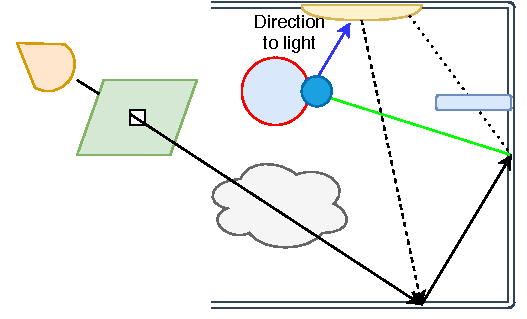
\includegraphics[width=\linewidth]{img/path_tracer_step5.pdf}
				\caption{Geometry hit, new direction points to light, add contribution and terminate}
		\end{subfigure}}
	\end{tabular}
	\caption{A visualization of a single walk in the path tracer}
	\label{fig:path_tracer_vis}
\end{figure}


\subsubsection{Other methods}
Path tracing is our main concern in this thesis due to its physically based and unbiased properties. Some of the other global illumination techniques are mentioned only briefly in the following description:

\begin{description}
	\item[Ray tracing]\cite{glassner1989introduction} Similar to the path tracing but there are no bounces from the surfaces --- simulates only reflections, refractions, scattering, etc. These days, real-time rendering is capable of ray tracing.
	\item[Photon mapping]\cite{jensen2001realistic} Two rays are traced independently --- from the camera and from the light source until termination occurs, then the radiance is computed based on their final positions. Faster in some scenarios but biased (does not have to converge to a correct solution).
	\item[Radiosity]\cite{sillion1994radiosity}Uses the finite element method instead of Monte Carlo. View independent, the light is traced from the source and bounced (possibly) to the viewer. Good for precomputations. 
\end{description}

\section{Spectral Rendering}

So far, we have considered the colors to be internally represented by a tristimulus color space during the rendering process. For the explanation purposes, let's assume RGB color space --- colors of all objects in the scene are defined in RGB, the path tracing step colors are RGB and the output color is RGB. In a large number of scenarios, this workflow is sufficient as we are capable of simulating a majority of the common aspects (e.g. optics) while keeping the rendering simple and robust. Unfortunately, the RGB color space is only a fraction of the visible gamut and has no notion of the light as electromagnetic radiation. Consequently, we are losing a significant amount of information, causing the colors to be at times inaccurate, and some phenomena completely impossible to render. 

Therefore, a new approach to the rendering has been introduced that internally represents the colors as a spectrum distribution function instead of a tristimulus color space --- the \emph{spectral rendering}. The core idea is to track and sample several wavelengths at once for each step of the path tracing and to perform the integration over all of them. We also generalize the BSDF to account for the wavelengths: $f_r(\lambda,\omega_i,\omega_o)$.

Most of the phenomena evaluated in this thesis are a direct consequence of the light's nature as electromagnetic radiation, hence the primary focus is placed on the spectral rendering.
The following sections are largely based on a publication by \citet{wilkie2002tone}.

\subsection{Color representation}

If the spectral rendering is desired, some representation of the spectral distribution functions needs to be implemented. While several techniques are feasible, it is often a matter of a simple trade-off between precision and performance. For example, sampling wavelengths uniformly each 5nm would yield significantly more accurate results than sampling only four wavelengths in total. However, such an approach might become unbearable in terms of speed and memory. Moreover, the spectral functions are usually quite smooth, therefore such dense sampling is mostly completely unnecessary. Some examples of these functions can be seen in \autoref{fig:spectral_color}.

A typical approach is to sample at larger ranges (more than 10 nanometers) and use basis functions for the representation~\cite{peercy1993linear}. More approaches and their details are briefly explained by \citet{wilkie2002tone}.

\begin{figure}[httpb]
	\centering
	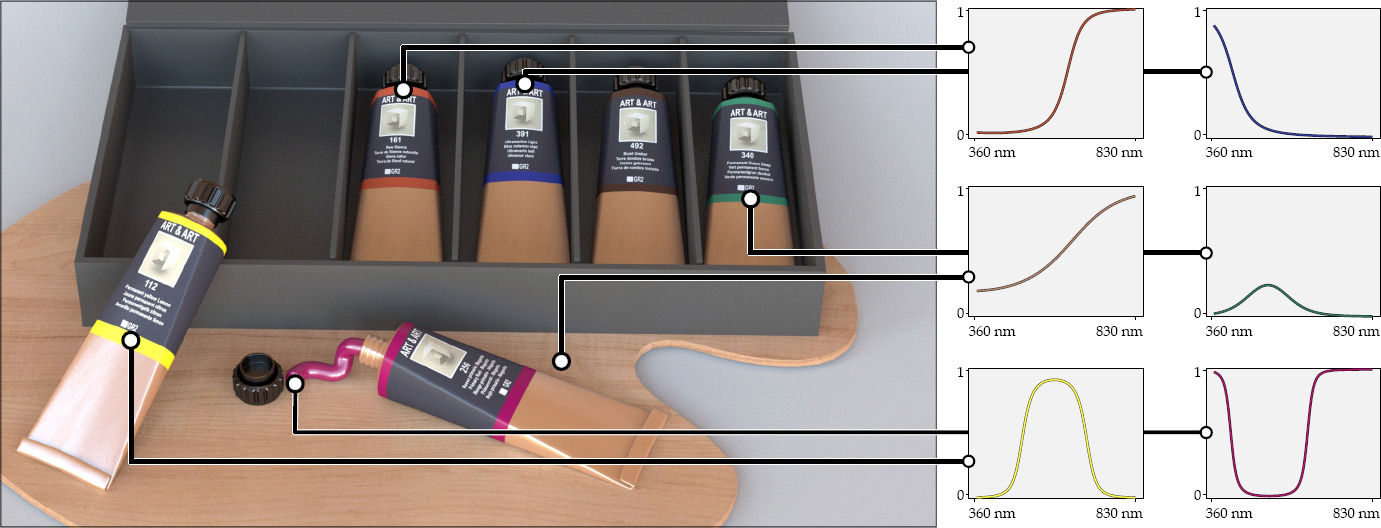
\includegraphics[width=.9\linewidth]{img/spectral_color.jpg}
	\caption{Spectral curves measured for different colors\cite{jakob2019low}.}
	\label{fig:spectral_color}
\end{figure}

\subsection{Advantages}

The spectral rendering presents the ability to reproduce the colors in a more photorealistic way. We might not see it at first, but the colors produced by a conventional RGB renderer tend to be slightly over-saturated as they do not account for the spectral characteristics of the light which might attenuate the final color. A comparison between the RGB and the spectral render of the same scene by Mitsuba2 is shown in \autoref{fig:compare_color}.

\begin{figure}[httpb]
	\begin{tabular}{cc}
		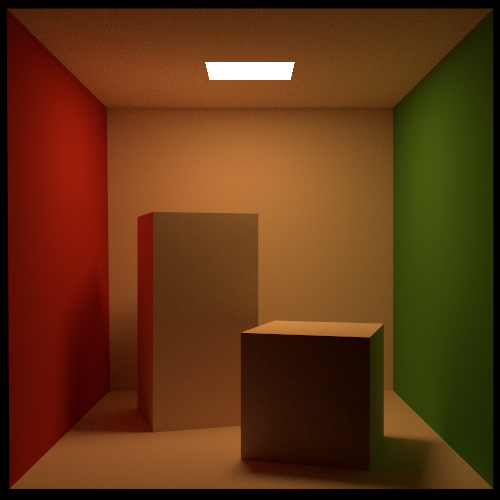
\includegraphics[width=.45\linewidth]{img/rgb.jpg}
		&
		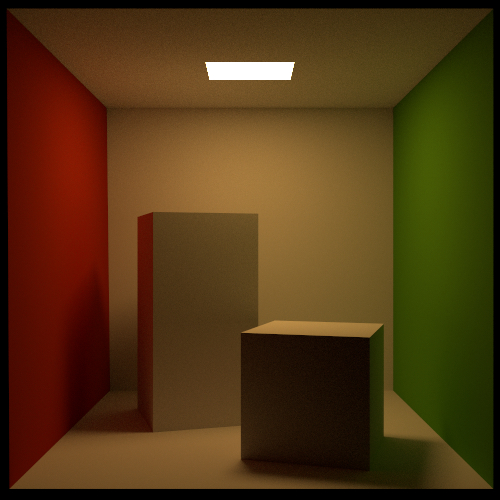
\includegraphics[width=.45\linewidth]{img/spectral.jpg}
	\end{tabular}
	\caption{A comparison between the RGB render (left) and the Spectral render (right) of the same scene by Mitsuba2~\cite{mitsubaWeb}}
	\label{fig:compare_color}
\end{figure}

Still, the biggest advantage is the possibility to reproduce some of the natural phenomena for which the tracing of multiple wavelengths is an absolute necessity. Namely, those are:
\begin{description}
	\item[Fluorescence] Absorption and re-emission of a different color
	\item[Dispersion] Splitting of the white light into its wavelength components via refraction
	\item[Polarisation] Change of the oscillation direction of a light wave 
	\item[Iridescence] Thin layer constructive/destructive light interference
\end{description}
They are explained in detail in \autoref{chap:appearance}.

\subsection{Disadvantages}

On the other side, the need to numerically integrate over multiple wavelengths introduces a problem of the chromatic noise. Fortunately, this has been effectively eliminated by the introduction of \emph{Hero Wavelength Spectral sampling}~\cite{wilkie2014hero}. Also, even though the performance is not a key factor, it worsens as well. 

Moreover, we assume that spectral images will not ever be properly displayable on the screens. Even the most modern monitors use a color space that is still smaller than the gamut of human-perceived colors. The only viable way is to store the distinct spectral bands as separate images. But, it is quite inconvenient to have multiple results instead of one as it does not correlate with the images that we capture in reality. Therefore, the rendering needs to have a well-done spectrum to final RGB conversion as the final image is still being displayed on an RGB monitor. Fortunately, the conversion is well-defined and fairly simple to implement.

Since the RGB gamut is only a subset of the visible spectrum, the situation gets significantly more complicated for the reversed conversion. As there exist infinitely many spectra for one RGB value, several techniques were proposed to convert the tristimulus to the spectral domain --- commonly called the \emph{spectral upsampling}. For those who may be interested in the details of the current development to the spectral upsampling, refer to the article by \citet{jakob2019low} which proposes a solution that is capable of converting full sRGB gamut with zero error.

It is also possible to simply map RGB values to their measured data. However, this requires a lot of manual work as the same "color" (reflective spectrum) might have to be measured for various lighting conditions and mapped accordingly.

There exist several reasons to integrate the spectral upsampling, mainly because the spectral values are a lot harder to obtain and to use. You need a specific device (spectrometer) that would measure the color values under a specific light and then use regularly distributed samples from it as an input. Because of the reproducibility of the RGB color space and its legacy usage (lots of existing textures are already defined in RGB), it is a lot more convenient to input the values of textures as RGB values, convert them internally to the spectral domain, and convert them back to the desired color space for the output image.
